


\documentclass{article}
\usepackage[utf8]{inputenc}

\usepackage{tabularx}


\usepackage{graphicx}
\graphicspath{ {./images/} }

\title{From BPMN to Permissioned blockchains: A model-driven approach}


\author{Nizar Hmain }




\date{August 2020}

\begin{document}

\maketitle





\begin{figure}[hbt!]
 \centering
\includegraphics[scale=0.2]{images/unicamqwe.jpg}
\end{figure}


Supervisor: Andrea Morichetta \newline
Assistant Phd: Alessandro Marcelletti


\pagebreak


\tableofcontents

\section{Abstract}

Blockchain technology’s innovative characteristics include decentralization, transparency, immutability, and automation. Our focus is to examine the various different facets of private data in enterprise blockchains such as Hyperledger Sawtooth and Quorum as well as integrating it with the ChorChain framework and extending it. 




\section{Introduction}

All Bitcoin transactions are public, traceable, and permanently stored in the Bitcoin network. This is maybe ideal for individuals making transactions but not fit for an enterprise use-case where multiple parties are not willing to share information globally. When having multiple organizations interacting with the blockchain, it would not be in their favor to disclose information that is private. Let's assume a simple scenario that involves two private companies and a public institution. The private companies may have a secure communication channel between them and the public institution, but they would not want to share that information with each other (if they were competitors for example). Disclosing sensitive information may reduce a competitive advantage and that would lead to some organization to never adopt a publicly open blockchain as part of their infrastructure. We aim at solving this issue by finding a way to guarantee the privacy of data through different methods (simply cryptography or targeted replication of data stores containing ledger information). \newline



\pagebreak

In order to understand the frameworks used in the rest of the work we must first go through the fundamentals of the blockchain

\section{Background and fundamentals}

A blockchain is essentially an append-only list of blocks that are linked using cryptography. Each block contains a cryptographic hash of the previous block, a timestamp and transaction data. \newline
Blockchain was invented by a person (or a group of people) anonymously using the alias of Satoshi Nakamoto in 2008. The identity to this day remains secret.

\subsection{The Data structure}

Blocks hold batches of valid transactions that are hashed and encoded into a Merkle tree. Each block includes the cryptographic hash of the prior block in the blockchain, linking the two. The linked blocks form a chain. This iterative process confirms the integrity of the previous block, all the way back to the original genesis block.

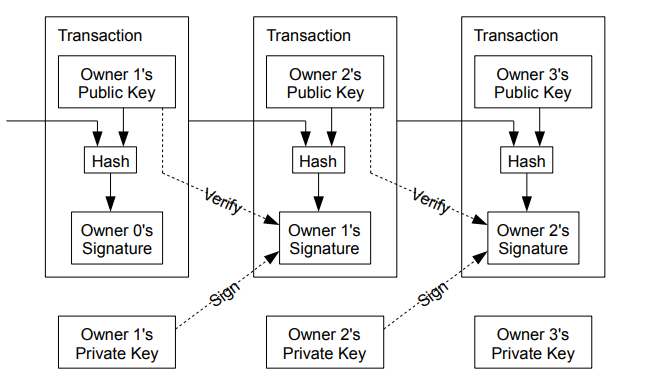
\includegraphics[scale=0.6]{images/satoshi_diagram.png}

The transaction are can be identified by a user's public key. \newline

\subsection{Merkle trees}

\includegraphics[scale=0.2]{images/merklee_tree.png}

A Merkle is a tree of hashes in which the leaves are hashes of data blocks. Nodes further up in the tree are the hashes of their respective children. The main difference from a hash list is that one branch of the hash tree can be downloaded at a time and the integrity of each branch can be checked immediately, even though the whole tree is not available yet. 

Finding out whether two different nodes have the same data or not can be efficiently done with the Merkle tree. You first have to compare the Top Hash value of the two nodes. If they are the same, then the two nodes have same data. For example, if you look at the picture above, when there are four nodes (L1, L2, L3, L4), you only need to check whether they have the same Top Hash or not. If the Top Hash is different and you want to know which data is different, you should compare Hash 0 with Hash1 and check which branch is different. By doing so, you will eventually find out which data is different.

\pagebreak

\subsection{Patricia trees}

\begin{figure}[hbt!]
 \centering
\includegraphics[scale=0.5]{images/patricia.png}
\end{figure}


Patricia trie is a data structure which is also called Prefix tree, radix tree or trie. Trie uses a key as a path so the nodes that share the same prefix can also share the same path. This structure is fastest at finding common prefixes, simple to implement, and requires small memory. Thereby, it is commonly used for implementing routing tables, systems that are used in low specification machines like the router.



\subsection{Modified Merkle-Patricia trees}

Ethereum uses a modified merkle-patricia tree that is a cryptographically authenticated data structure used to store (key, value) pairings. It provides the efficiency of $ O(log(n))$ for inserting, retrieving and removing items. There are three kind of nodes. \newline

- Branch nodes: The first item is the hash of hashes stored in child nodes. The last sixteen items are child nodes, and it corresponds to each of the possible nibble values for the keys at this point in their traversal.

- Domain nodes: They have eighteen items. The first item is the hash of hashes stored in child nodes. The extra item stores the information of address bound with domain. The other sixteen items are the same as branch nodes.

- Certificate nodes: are leaf nodes in the bottom of the tree that only store two items, the certificate and its hash.

\begin{figure}[hbt!]
 \centering
\includegraphics[scale=0.4]{images/mpt.png}
\end{figure}

\pagebreak


\subsection{Cryptogpraphy}

The concept of a global state in a blockchain means that anyone can add a new entry to it. That comes with a small complication about the differentiation between users.
We must add something that is unique to each entity or user. If Alice wants to send a transaction to Bob. We must make sure that it's unfeasable for anyone else to forge this transaction in her name. This is where the concept of digital signatures comes in and public asymmetric key cryptography. Asymmetric means that each entity selects a key pair consisting of a private key and a related key. The entity maintains the secrecy of the private key which it uses for signing messages, and makes authentic copies of its public key available to other entities which use it to verify signatures. Ideally, a digital signature scheme should be existentially unforgeable under chosen-message attack. Informally, it asserts that an adversary who is able to obtain entity $A$'s signatures for any messages of its choice is unable to successfully forge $A$'s signature on a single other message.

\[ Sign(Message, sk) = Signature  \]
\[ Verify(Message, Signature, pk) = True / False  \]

Both bitcoin and Ethereum us an  Elliptic Curve Digital Signature Algorithm (ECDSA) which is a variant of Digital Signature Algorithm (DSA) which uses elliptic curve cryptography.



\subsection{Elliptic Curve}

Elliptic Curve forms the foundation of Elliptic Curve Cryptography. It’s a mathematical curve given by the formula — $y² = x³ + a*x² + b$, where $a$ and $b$ are constants. Following is the diagram for the curve $y² = x³ + 1$ \newline


You can observe two unique characteristics of the above curve:

\begin{itemize}
  \item The curve is symmetric about the X-axis. Every point on the curve lying above the X-axis has a reflection below it
  \item If a non-vertical line is drawn, it can intersect the curve in at most 3 points
\end{itemize}


\begin{figure}[hbt!]
 \centering
\includegraphics[scale=0.4]{images/trapdoor.png}
\end{figure}


In the above diagram, two points $P$ and $Q$ are chosen. The line joining these two points meets the curve at point $R$. Reflection of point $R$ on the X-axis is $R’$.
The process can now be repeated with the points $P$ and $R’$. As illustrated below, the addition of these two points will result in $S’$ on the curve above the X-axis. This process can be repeated and is known as Elliptic Curve scalar multiplication or point multiplication.

Trapdoor function forms the cornerstone of Public Key Cryptography. In simple words, it’s a function that is easy to compute in one direction but computationally difficult in the opposite direction.
As a simple example is you need to find two prime numbers whose product is $39203$. You will begin with the number $2, 3, 5, 7,$ until you find a prime number that divides $39203$. But, if given that one of the numbers is $197$, you can find the other by entering $39203 / 197 = 199$
This function in the above example can be made difficult by increasing the number of digits. Given two prime numbers, you can easily multiply and find the result. Yet, given a result, it becomes difficult (depending on the digits) to find two prime numbers such that their product equals the result.
The same concept is extended to an Elliptic Curve. We choose a point on the curve and multiply with itself $n$ times. We can easily find the location of destination point given the starting point and $n$. If you are only given the destination point and the starting point, it becomes difficult to find the value of $n$.

In the above diagram, if we start with $P$ and $n=2$, we can reach $S’$. However, given the points $P$ and $S’$, it’s nearly impossible to calculate the value of $n$.



A pre-determined point is selected on the curve. This point is known as the Generation point $(G)$. The private key is randomly generated and corresponds to the number 
$n$. The generator point $(G)$ must be multiplied with itself $n$ times to find point $K$, which is the public key. \newline

Bitcoin uses the secp256k1 which is $y² = x³ + 7$. \newline

One reason for using ECDSA as opposed to RSA, is that ECDSA has equivalent security to RSA while using smaller key sizes. 256-bit public key's computational complexity in ECDSA translate to roughly same the computational complexity of a 3072-bit public key for RSA.


\subsection{ECDSA}

The Elliptic Curve Digital Signature Algorithm offers a variant of the Digital Signature Algorithm which uses elliptic curve cryptography. The original Digital Signature Algorithm was specificed in a U.S. Governement Federal Information Processing Standard (FIPS) called the DSS[70]. Its security is based on the computational intractability of the discrete logarithm problem (DLP) in prime-order subgroups of $Z_p$. Koblitz and Miller invented the ECC (Elliptic curve cryptosystems) and the subgroup of $Z_p$ was replaced by the group of points on an elliptic curve over a finite field. The mathematical basis for the security of elliptic curve cryptosystems is the computational intractability of the elliptic curve discrete logarithm problem (ECDLP).

There are six parameters in total for the signature generation algorithm.


\begin{itemize}
    \item Curve: the elliptic curve field and equation used
    \item G: elliptic curve base point, a point on the curve that generates a subgroup of large prime order n
    \item n: integer order of $G$, meaning that $n$ x $G$ = $O$, where $O$ is the identity element
    \item $d_A$: the private key (randomly selected)
    \item $Q_A$: the public key (calculated by the elliptic curve)
    \item $m$: the message to send
\end{itemize}


For Bob to authenticate Alice's signature, he must have a copy of her public-key curve point $Q_a$. Bob can verify $Q_a$ is a valid curve point as follows:

\begin{itemize}
  \item Check that $Q_a$ is not equal to the identity element $O$, and its coordinates are otherwise valid.
  \item Check that $Q_a$ lies on the curve
  \item Check that $n$ x $Q_A$ = $O$
\end{itemize}

After that, Bob folows theses steps:

\begin{itemize}
  \item Verify that $r$ and $s$ are integers in $[1, n - 1]$. If not, the signature is invalid.
  \item Calculate $e = HASH(m)$, where $HASH$ is the same function used in the signature generation.
  \item Let $z$ be the $L_n$ leftmost bits of $e$.
  \item Calculate $u_1 = zs^{-1} mod n$ and $u_2 = rs^{-1} mod n$
  \item Calculate the curve point $(x_1, y_1) = u_1$ x $G + u_2$ x $Q_A$. If $(x_1, y_1) = O$ then the signature is invalid.
  \item The signature is valid if $r := x_1 (mod n)$, invalid otherwise.
  
\end{itemize}




\subsection{Common loopholes}

Public key cryptography stops someone from copying transactions. But it does not stop some malicious actor from copying exactly the same message with it's signature and replicate the same message. In order to implement a forgery defence mechanism we need to introduce some unique variable in the transaction. Usually by appending a $tx_id$


\begin{itemize}
  \item Alice sends Bob 20 dollars = the signature is $001101$
  \item Alice sends Bob 20 dollars = the signature is $001101$
\end{itemize}

When we append transaction ids to the packet

\begin{itemize}
  \item $tx=1$ Alice sends Bob 20 dollars = the signature is $001101$
  \item $tx=2$ Alice sends Bob 20 dollars = the signature is $100001$
\end{itemize}


On the other hand verifying a transaction requires you to know all the history of transactions up to that specific point. That's how overspending is stopped.

\section{Decentralized / Distributed nature }


\begin{figure}[hbt!]
 \centering
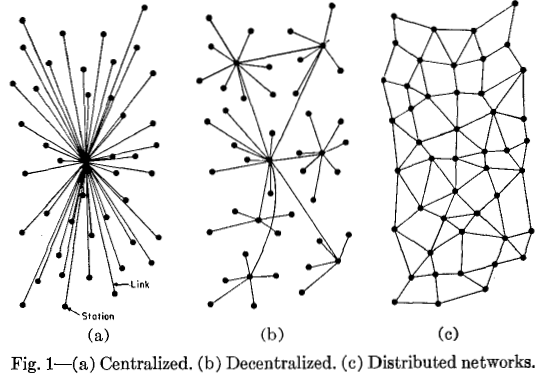
\includegraphics[scale=0.5]{images/networks.png}
\end{figure}



While a blockchain is inherently distributed (meaning that many parties hold copies of the ledger), it is not inherently decentralized. Whether a blockchain is centralized or decentralized simply refers to the rights of participants on the ledger, and is therefore a question of design.


By storing data accross its peer-to-peer network, the blockchain eliminates a number of risks that come with data being held centrally.

It has essentially no central point of failure. A public key represents an address on the blockchain while a private key is analogous to a password that gives its owner access to their digital assets or the means to otherwise interact with the various capabilities that blockchains now support. It is generally considered incorruptible (more on that later).


Ethereum addresses are 160 bit hashes, meaning there are $2^{160}$ possible hashes. Per the birthday problem, the chance of a collision rises to 50 percent when there are about $2^{80}$ accounts created. \newline

To give you an idea of how unlikely that is, if every person on earth spent all their time doing nothing but generating Ethereum accounts, and they generated one every second, they'd only generate about $2^{57}$ of them. To generate $2^{80}$ and reach a 50 percent probability of finding a collision, they would need to keep on generating one per second for about 8 million years. This is also one way that account security is enforced, if you can generate a duplicate key hash, you can also steal someones assets.


Growth of a decentralized blockchain is accompanied by the risk of centralization because the computer resources required to process larger amounts of data become more expensive therefore less accessible.

There are at least four different types of blockchains:


\begin{itemize}
  \item Public blockchains with no access restrictions, anyone can send transactions to it as well as become a validator. There are usually economic incentives for those who secure them. (Bitcoin and Ethereum)
  \item Private blockchains are permissioned. Validators and participants access is restricted
  \item Consortium blockchains which are hybrid and are usually inter-organizational
\end{itemize}

Our focus is primarly on the consortium blockchains. (Hyperledger and Quorum). The most important difference to remember is that a blockchain is just one type of distributed ledger. Allthough a blockchain is a sequence of blocks, distributed ledgers do not require such a chain. Furthermore, distributed ledgers do not need proof of work and theoretically offer better scaling options.

\subsection{Peer-to-peer discovery mechanisms}

Since it is a decentralized system, there needs to be a way to find out about other nodes in the network. Ethereum for example uses a Distributed hash table that provides a lookup service similar to a standard hash-table. BitTorrent and Gnutella initially motived DHT, which took advantage of resources distributed accross the Internet to provide a single useful application. It is an essential piece of any blockchain. \newline

The first generation p2p file sharing networks relied on a central database to co-ordinate look ups on the network. Second generation p2p used flooding to locate files. Third generation p2p uses Distributed hash tables for lookups. \newline

Kademia is the protocol used by Ethereum, it uses a distance calculation between two nodes. The distance is computed as $XOR$ of the two node IDS taking the result as an unsigned integer number. 

The $XOR$ was chosen because it acts as a distance function between all node IDS:




\begin{itemize}
  \item The distance between a node and itself is zero
  \item It is symmetric: The distance between $A$ and $B$ and from $B$ to $A$ are the same
  \item given $A$ $B$ $C$ are vertices of a triangle, then the distance from $A$ to $B$ is shorted than (or equal to) the sum of the distance from $A$ to $C$ + $C$ to $B$
\end{itemize}


Kademlia uses routing tables that consist of a list for each bit of the node ID. A list has many entries. Every entry in a list holds the necessary data to locate another node. The data in each list entry is typically the IP address, port, and node ID of another node. Every list corresponds to a specific distance from the node. Nodes that can go in the $n^th$ list must have a differing $n^th$ bit from the node's ID.

\begin{figure}[hbt!]
 \centering
\includegraphics[scale=0.4]{images/kademlia.png}
\end{figure}

Consider the simple network in the following figure. The network size is $2^3$ or eight maximum keys and nodes. There are seven nodes participating. The node we will consider is node six (110 in binary). There are three $k$-buckets for each node in this network. Nodes zero, one and two are condidates for the farthest $k$-bucket, nodes four and five are placed. Finally, the third $k$-bucket can only contain node seven. Each node knows its neighbourhood well and has contact with a few nodes far away which can help locate other nodes further away. \newline

Nodes that have been connected for a long time in a network will probably remain connected for a long time in the future. Because of this statistical distribution, Kademlia selects long connected nodes to remain stored in the $k$-buckets. This increase the number of known valid nodes at some time in the future and provides for a more stable network.


A node that would like to join the net must first go through a bootstrap process. In this phase, the joining node needs to know the IP address and port of another node (the bootsrap node). If the joining node has not yet participated in the network, it computes a random ID number that is supposed not to be already assigned to any other node. It uses this ID until leaving the network.


\subsection{Consensus}

A distributed ledger protocol can be summarized as a secure distributed protocol that achieves certain task satisfying targeted consistency (typically atomicity) and liveness semantics. However verifying and establishing trust in the security, consistency and livness semantics of a blockchain protocol is challenging. A blockchain is a distributed database holding a continuously growing list of records, controlled by multiple entities that may not trust each other. Records are appended to the blockchain in batches or blocks through a distributed protocol executed by the nodes powering the blockchain. Each block contains a cryptographic hash of the previous block, which fixes all existing blocks and embeds a secure representation of the complete chain history into every block. Naturally some nodes might crash, have malicious intentions or the network communication may simple become interrupted. The nodes are therefore required to run a fault-tolerant consensus protocol to ensure that they all agree on the order in which entries are appended to the blockchain. A blockchain protocol ensures this by replicating the data and the operations over multiple nodes. Replication may have various functions, but blockchains only replicate data for durability, not scalability. 
In theory, all nodes validate the information to be added to the blockchain; this feature increases the trust of all nodes in that the blockchain as a whole. The Paxos algorithm is the classic consensus protocol for state machine replication in environments that admit crash failures, and its single-decree version (SD-Paxos for short) allows a set of distributed nodes to reach an agreement on the outcome of a single update. Nakamoto's Bitcoin paper does not explicitly mention the state-machine replication paradigm, it instead establishes consensus on one shared ledger based on votes with each node's CPU power expressing their acceptance of valid blocks by working on extending them and rejecting invalid blocks by refusing to work on them.



\subsection{Zero Knowledge Proof}

A zero-knowledge proof (abbreviated as ZKP) is a cryptographic method that allows a party to demonstrate to another party that a statement is true without conveying any additional information. Suppose Alice wishes to prove to Bob the statement \textit{"I (Alice) own 30 bitcoins"}. A simple method for Alice to do so is to point to 30 coins on the block chain and, for each of them, sign a message ("this is Alice's"), using the secret key that controls that coin. Alas, this method leaks knowledge to Bob, by identifying which coins are Alice's. A zero-knowledge proof of knowledge allows Alice to achieve the same goal without revealing information to Bob (beyond the fact that she knows some secret keys that control 30 coins). Crucically, such proofs can be obtained for any statement that can be verified to be true by use of an efficient computation involving auxiliary inputs such as passwords (these are also referred to as "NP statements"). Intuitively, an NP problem is one that if you have a solution that is computationally easy to verify, but it is not know if it is computationally easy to find. Their connection with zero-knowledge proofs comes from the 1987, Goldreich, Micali and Widgerson paper that proves that all NP problems have zero knowledge proofs.

It basically allows for example you to proove that your bank balance is between a certain range without actually precisely revealing your balance. There are mainly three properties for a ZKP:


\begin{enumerate}
    \item Completeness: If the statement is true, an honest verifier will be convinced by an honest prover.
    \item Soundness: If the statement is false, no dishonest prover can convince an honest verifier.
    \item Zero-Knowledge: If a statement is true, no dishonest verifier learns anything other than the fact that the statement is true.
\end{enumerate}

There are two types of ZK proofs

\begin{enumerate}
    \item Interactive: For each verification, a demonstration is needed. As you can tell this might not really be viable in a blockchain context (since the numbers of participants could potentially be fairly high, the amount of verification and demonstration would quickly become a performance bottleneck). 
    
    \item Non-Interactive: The prover can show the result, and another party (the verifier) can verify the proof themselves. (this fits quite well within our blockchain and distributed network context).
\end{enumerate}

Zk-Snarks stands for Zero-Knowledge Succinct Non-interactive Argument of Knowledge are ZKP-variants. They require no interaction between provers and verifiers. The most appealing example of ZK-SNARK is its application in Zcash. Ethereum also plans to roll-out ZK-SNARKS on its upcoming phase (Metropolis). ZK-SNARKS are generic and they can verify any function which is particularly relevant for Ethereum since it provides the Turing-complete EVM, allowing developers to build any type of logic.

We should now discuss the non-interactivity which is the crucial aspect in our current blockchain context. The interactive version considers a proof valid only for the original verifier and nobody else and that's due to these different reasons:

\begin{enumerate}
    \item The verifier could collude with the prover and disclose those secret parameters $s$, $α$ which allows to fake the proof
    \item The verifier can generate fake proofs himself for the same reason
    \item The verifier has to store $α$ and $t(s)$ until all relevant proofs are verified, which allows an extra attack surface with possible leakage of secret parameters
\end{enumerate}

Therefore a separate interaction with every verifier is required in order for a statement to be proven. It is quite inefficient when one needs to convince many parties simultaneously or permanently. That is the main reason why secret parameters need to be reusable, public, trustworthy and infeasible to abuse. In order to achieve that the concept of Cryptographic pairings (also called bilinear map) are used. This mathematical construct also makes use the previously discussed elliptic curves to achieve these properties.








\subsection{Proof Of Work}

Proof of Work is a consensus model introduced by Satoshi Nakamoto as the backbone of the system. PoW protocol needs the adoption of diverse conventions, relative for instance to the size of each "block" which bother transactions waiting for validation, the bounty reward of validators (called "miners") which consists in the Bitcoin case in the monetary creation, the reward amount adjustment in time, and the money supply limit. It is the combination of cryptography and computational power that creates consensus and ensures the authenticity of data recorded on the blockchain. To prove that a block is valid and that work has been done, the nodes in the network (called miners) use their computational power to validate transactions (i.e verify that a sender has enough funds and is not double-spending) and most importantly compete with each other in a race to solve cryptographyic problems imposed by the protocol. This process is called mining. There are two main incentives for miners to join the race: the first miner to find a solution is rewarded with a bounty defined by the protocol and gets to collect all the transaction fees associated to the transactions that he / she included in the block. When a miner finds a solution he / she creates a block $X$ by including the hash of the previous block, the timestamp and transactions. The miner broadcasts the newly created block $X$ to the network and other miners verify the transactions and validate the block. The block is considered as legitimate when other miners continue working on extending the chain from block $X$. When a chain splits, miners should always choose the longest chain since it has the most work done. Miners can work on multiple chains if they whish to but to the detriment of dividing their computational power. \newline

Althought it resembles a lottery, the computational power that a miner possesses plays a deterministic role in the PoW protocol as the bigger the capacity to generate guesses increases. It is considered a resource-intensive consensus protocol, time and energy serve as proofs that work has been done. in 2014, the power consumed by the Bitcoin network was equal to Ireland's electricity consumption. The future of this protocol remains unclear, particularly because it was not imagined to manage the speculative asset that became Bitcoin.



\subsection{Proof Of Stake} 

An alternative to the PoW is the Proof of Stake (PoS) protocol. It confers
decision power to minters that actually have a stake in the system. Unlike the
PoW in which everyone can become a miner, the network is restricted . Ownership of a currency or having a deposit in the network allow the nodes to participate in the minting process i.e. to validate transactions and create blocks. No computational power is required to solve cryptographic puzzles like in the PoW scheme. There are no monetary rewards. Validators collect fees from users and are paid from them as an usual intermediary. Since validators only get transaction fees, the scenario in which validators create empty block can be avoided as they are incentivised to include a maximum number of transactions to maximize their gains. The money supply must be issued since the beginning. However the problem of an initial fair coin distribution arises. Additional balancing mechanisms are necessary to mitigate the risk of rich validators getting richer. There are some solutions to that problem like stochastic PoS minting process. The Stochastic minting process uses the duration of an unspent coin and determines its coinage (i.e a person holding 4 coins for 10 days will have accumulated 40 coin-days and will have 4 times more chance to generate profit than a person who has 10 coin-days). Once a miner is chosen to create a block, his coinage resets to zero and he must wait again to accumulate coinage. The minting process is designed to yield around one percent profit per year.


\subsection{Byzantine fault tolerance}


It is the property of a system being able to resist the problems  and failures derived from the byzantine generals problems. A BFTS is a system that continues to work when nodes are malicious or fail to communicate. This is a crucial property for blockchains, as networks are always under constant fire from malicious and external threats.
A byzantine fault is a condition of a computer system where components may fail and there is imperfect information on whether a component has failed. The term takes its name from the "Byzantine Generals Problem" \newline
In its simplest form, the generals must decide only whether to attack or retreat. Some generals may prefer to attack, while others prefer to retreat. The important thing is that every general agrees on a common decision, for a halfhearted attack by a few generals would become a rout, and would be worse than either a coordinated attack or a coordinated retreat. The problem is complicated further by the generals being physically separated and having to send their votes via messengers who may fail to deliver votes or may forge false votes. Allthought the problem is formulated in the analogy as a decision-making and security problem, in electronics, it cannot be solved simply by cryptographic digital signatures, because failures such as incorrect voltages can propagate through the encryption process. Thus, the perception of correctness is altered when a node is checking another node and that prevents from forming a consensus as to whether the component is faulty or not.

Given a system of $n$ components, $t$ of which are dishonest, and assuming only point-to-point communication between all the nodes.

If node $A$ tries to broadcast value $x$, the other nodes are allowed to communicate with each other and verify the consistency of $A$'s broadcast, and eventually settle on a common final value $y$ \newline


Thy system is resistant to a Byzantine fault if a node $A$ broadcast a value $x$:

\begin{itemize}
  \item If $A$ is honest, then all honest components agree on the value $x$
  \item In any case, all honest components agree on the same value $y$
\end{itemize}


\begin{center}
\begin{tabular}{ | m{4cm} | m{2cm}| m{2cm} | m{2cm} | m{2cm} | } 
\hline
Which faults are tolerated & Special-node & $t<n/2$ crash & special-node subverted & $f<n/3$ nodes subverted \\ 
\hline
Fabric/Kafka & . & yes & . & no \\ 
\hline
Fabric/PBFT & . & yes & . & yes \\ 
\hline

Sawtooth PoET & trusted HW & yes & trusted HW & no \\ 
\hline


Tendermind & . & yes & . & yes \\ 
\hline

Corda/Raft & . & yes & . & no\\ 
\hline
Corda/BFT-SMaRt & . & yes & . & yes \\ 
\hline

Quorum/QuorumChain & no & yes & no & no \\ 
\hline

Quorum/Raft & . & yes & . & no \\ 
\hline

Quorum/PBFT & . & yes & . & yes \\ 
\hline


\end{tabular}
\end{center}

Table1: Trusted HW: assumes trusted hardware available from only one vendor. '.' states that no special node exists in the protocol


\section {Ethereum & Smart Contracts: Enabling a Decentralized Future}

In order to follow up with Quorum and the Hyperledger, we ought to understand how Ethereum works, since a lot of the work is based around this ecosystem.

\subsection{Bitcoin vs Ethereum}

Bitcoin is a single application while Ethereum is an application layer. If Bitcoin is email, Ethereum is the World Wide Web.
Ethereum is account based, bitcoin instead is utxo based. UTXO stends for (Unspent transaction output). Ethereum has a native asset called ether (ETH). It represents the basis of value in the ETH ecosystem and it is needed to align incentives, given to miners as a reward for finding new blocks. Eth has a smart contract platform that is complex, feature-rich and a turing complete scripting language. We can use this approach to define arbitrary computations on the blockchain. \newline Bitcoin has a similar concept with colored coins as it was designed to be layered on top of Bitcoin. Using colored coins, bitcoins could be "colored" with specific attributes. This effectively turns them into tokens, which can be used to represent anything. \newline

This gives us the following benefits

\begin{enumerate}
    \item Virtually any kind of asset or contract can be represented using them.
    \item They can be transferred digitally to a new owner with no need for central authorization, which has implications for ease of use, efficiency and availability
    \item Properly used, ownership of these colored coins can be made anonymous, while still enjoying the benefits of ownership
\end{enumerate}

There are however drawbacks using them

\begin{enumerate}
    \item Scalability is further more decreased. Every transaction carries the marginal cost of being received, verified and stored by every node on the network.
    \item Funding hashing becomes a problem. Since the cost of hashing is amortized over all transactions, it is essentially a bargaining game between miners and users, which unconstrained would lead to a race to the bottom. With colored coins, the network is unable to determine the value of the transactions and charge accordingly.
    \item Legal concerns such as uncertainty about security trade regulations or specific unsavory assets.
\end{enumerate}

Both Bitcoin and Ethereum have scripting capabilities. They are however targeted different use cases. Ethereum does not revolve primarily around the ether, the currency acts almost as a side effect to its incentive-aligned smart contract platform. The ethereum ecosystem plans to change its protocol from Proof Of Work to Proof of Stake. \newline
The block creation times between the two are quite different, every 12 seconds an ethereum block is mined, while it takes around 10 mins for bitcoin. \newline
Ethereum uses a modified version PoW, it uses Ethash instead of Sha256 as its hashing algorithm. The advantage is that Ethash is ASIC resistant. ASIC-resistance is the property of a cryptocurrency that is "immune" to ASIC mining. ASICs are integrated circuits that are created to serve a specific use case, performing a particular computing task (EFF DES cracker was an ASIC machine built exclusively to brute force DES encryption). It would not be economically feasible to create specialised chips. \newline

Ethereum is account based, which essentially means that ownership is typically in the form of an account that has an address and some balance in it. You can create a new account even if you are disconnected from the network. Account uniqueness is almost certainly guaranteed. Address in Ethereum are 160 bit hashes, meaning there are $2^160$ possible hashes. According to the birthday problem the chance of collision rises to 50 percent when there are about $2^80$ accounts created. To give you an idea of how unlikely that is, if every person on earth spent all their time doing nothing but generating Ethereum accounts at a rate of one account per second, they would only be able to generate about $2^57$ of them. In order to get to that 50 percent collision chance, they would need to keep generating at that rate for about 8 million years. \newline

Bitcoin on the other hand does not represent accounts. It uses instead the private keys of some UTXO and that is the defining factor in bitcoin ownership.



\subsection{Smart Contracts}

A contract is an agreement between two unstrusting parties than can later be action-enforced by a court of law. A smart contract is encoding that contract in a digital form. Without ETH we would need a trusted entity, we can remove that trusted party and replace it with the network. The smart contract runs in a global distributed network. The smart contracts are executed by the network itself. Every single node executes essentially the code. It is parallelly redundant whereas every node is updating the same state at the same time. This ensures that no one violates the contract. They are analogous to autonomous agents that live in the blockchain and they don't do anything until we give them an external stimuli. There are several example use cases:



Two type of accs in eth: Externally (person, corporation), can send tx to other accounts. Contract accs also have balanced but also associated contract code. Code execution is triggered by transactions or messages (function calls) received from other contracts or EOAs. Contracts have persistent storage.
The network state 
bitcoin: unspent transaction output set
eth: account state (every account's state)

rational of eth using this acc model instead of the utxo model:
- space savings: nodes only need to update each account's balance instead of storing every UTXO
- More intuitive: smart contracts are easier to program when transferring between accounts with a balance than constantly updating a UTXO set to compute user's available balance.



\begin{enumerate}
\item - store and maintain data: token currency or organization's membership, domain,
\item - managing trust relationships: financial contracts, escrow, insurance.
\item - Provide functions to other contracts: analogous to software libraries.
\item - Complex Authentication: multisignature access
\end{enumerate}

\subsection{Ethereum Virtual Machine}

The Ethereum Virtual Machine(EVM) is the runtime environment for smart contracts in Ethereum. It is a 256-bit register stack, designed to run the same code exactly as intended. It is the fundamental consensus mechanism for Ethereum. The formal definition of the EVM is specified in the Ethereum Yellow Paper. Ethereum Virtual Machines have been implemented in C++, C#, Go, Haskell, Java, JavaScript, Python, Ruby, Rust, Elixir, Erlang, and soon, WebAssembly. \newline

Design goals of the EVM: 

\begin{enumerate}
    \item Simplicity: op-codes should be as low-level as possible.
    \item Space Efficiency: EVM assembly should be as compact as possible.
    \item Determinism: Same input state should always yield the same output state. (regardless of cpu architecture for example arm or x86).
    \item Specialization: modular arithmetic used in custom cryptography.
\end{enumerate}



\begin{figure}[hbt!]
 \centering
\includegraphics[scale=0.5]{images/evm.png}
\end{figure}


Smart contracts are high-level programming abstractions that are compiled down to EVM bytecode and runs on the EVM. It is similar to the JVM. Every ethereum node runs the EVM as part of its block verification procedure. They can be written in a multitude of languages, Solidity (similar to C and Javascript), Serpent (similar to Python), LLL (low-level Lisp-like language). One issue related to the usage of smart contracts on a public blockchain is that bugs, including security holes, are visible to all but cannot be fixed quickly. One example of this is the 17 June 2016 attack on The DAO, which could not be stopped or reversed (a soft fork happened). There is a lot of ongoing research on formal verification to express and prove non-trivial properties. There are open source tools like Slither that help analyze Solidity source code, it effectively runs a suite of vulnerability detectors, it enables developers to find vulnerabilities, enhance their code comprehension and quickly prototype custom analyses.












\pagebreak


\section{References}




\begin{enumerate}
  \item Satoshi Nakamoto; Bitcoin: A Peer-to-Peer Electronic Cash System
  \item Fromknecht, Velicanu, Yakoubov; A NameCoin Based Decentralized Authentication System.
  \item Hammerschmidt; Consensus in Blockchain Systems. In Short.
  \item Cachin, Vukolic; Blockhain Consensus Protocols in the Wild
  \item Garcia-Perez, Gotsman, Meshman, Sergey. "Paxos Consensus, Deconstructed and Abstracted Extended Version"
  \item Castro, M.; Liskov, B. (2002). "Practical Byzantine Fault Tolerance and Proactive Recovery". ACM Transactions on Computer Systems. 
  \item  Johnson, Menezes, Vanstone, "The Elliptic Curve Digital Signature Algorithm" 
  \item Ongaro, Ousterhout. In Search of an Understandable Consensus Algorithm (Extended Version).
  \item O’Dwyer, K. J., and Malone, D. (2014). Bitcoin mining and its energy footprint. Paper
presented at the 25th IET Irish Signals & Systems and China-Ireland International Conference on Information & Communities Technologies (ISSC/CIICT), Limerick, June 26-27
  \item Seang, Torre; Proof of Work and Proof of Stake consensu protocols: A blockchain application for local complementary currencies.
  \item Maksym Petkus;Why and How zk-SNARK Works: Definitive Explanation
  \item Koens, Ramaekers, van Wijk; Efficient Zero-Knowledge Range Proofs in Ethereum
  \item https://medium.com/@VitalikButerin/zk-snarks-under-the-hood-b33151a013f6
  \item Ben-Sasson; Chiesa; Garman; Green; Miers; Tromer; Virza; Zerocash: Decentralized Anonymous Payments from Bitocin [2014]
  \item Goldreich; Micali; Widgerson; Proofs that yield nothing but their validity or all languages in NP have zero-knowledge proof systems.
  \item Matthew Green; Zero Knowledge Proofs: An illustrated primer.
  \item Vitalik Buterin; A Next generation smart contract & decentralized application platform [2018]
  \item Gavin Wood; Ethereum Yellow paper: A secure decentralised generalised transaction ledger
  \item Wikipedia; https://en.wikipedia.org/wiki/Ethereum
  \item Wang, Lahiri, Chen, Pan, Dillig, Born, Naseer; Formal Specification and Verification of Smart Contracts in Azure Blockchain
  \item Slither, solidity source analyzer; [https://github.com/crytic/slither]
  \item Mastering Bitcoin: Unlocking Digital Cryptocurrencies, Andreas Antonopoulos, 2014
  \item Meni Rosenfeld; Overview of Colored Coins [2012]
  \item https://en.wikipedia.org/wiki/EFF_DES_cracker
  \item https://en.wikipedia.org/wiki/Birthday_problem
  
  
  



\end{enumerate}


\end{document}









